\section{Empirical Analysis}\label{sec:eval}


In this section, we use empirical analysis to verify our theoretical findings regarding tensor core performance on memory-bound kernels. We conduct experiments across multiple hardware platforms, detailed in Table~\ref{tab:env}, to systematically evaluate the performance relationship between tensor core and CUDA core implementations.


% In this section, we use empirical analysis to debunk the tensor core's performance advantage in memory-bound kernels. The hardware platforms that we used are summarized in Table~\ref{tab:env}.
\begin{table}[t]
    \caption{Specifications of the experimental platforms.}
    \label{tab:env}
    \vspace{-14pt}
    \centering
    \footnotesize
    \begin{tabular}{|l|c|c|c|}
    \hline
    \multicolumn{2}{|c|}{\textbf{Metric}}             & \textbf{A100-80GB} & \textbf{GH200} \\\hline
    \multicolumn{2}{|c|}{\textbf{CUDA Version}}             & 12.1 & 12.6\\\hline
    \multicolumn{2}{|c|}{\textbf{L2 Cache (MB)}}        & 40               & 50           \\\hline
    \multicolumn{2}{|c|}{\textbf{Memory Bandwidth (TB/s)}}        & 1.94               & 4.00           \\\hline
    \multirow{2}{*}{\textbf{FP64 Peak (TFLOPS)}} &\textbf{CUDA Core}&  9.7    &  34.0  \\
                                            &\textbf{Tensor Core}& 19.5   &  67.0   \\\hline
    % \multirow{2}{*}{\textbf{Balance}}       &\textbf{CUDA Core}& 5.0       &  8.5   \\
    %                                         &\textbf{Tensor Core}& 10.0      &  16.8  \\\hline
    % 
    \end{tabular}
    
\end{table}

% \begin{table}[t]
%     \centering
%     \footnotesize
%     \renewcommand{\arraystretch}{1.3} % Adjust row spacing
%     \setlength{\tabcolsep}{5pt} % Adjust column spacing
%     \begin{tabular}{@{}llcc@{}}
%     \toprule
%     \multicolumn{2}{l}{\textbf{Metric}}               & \textbf{A100-80GB} & \textbf{GH200} \\ \midrule
%     \multicolumn{2}{l}{\textbf{CUDA Version}}         & {12.1}      & {12.6}  \\
%     \multicolumn{2}{l}{\textbf{L2 Cache (MB)}}        & {40}        & {50}    \\
%     \multicolumn{2}{l}{\textbf{Memory Bandwidth (TB/s)}} & {1.94}   & {4.00}  \\ \midrule
%     \multirow{2}{*}{\textbf{Peak (TFLOPS)}} 
%         & \textbf{CUDA Core}    & {9.7}     & {34.0}  \\
%         & \textbf{Tensor Core}  & {19.5}    & {67.0}  \\ 
%     \bottomrule
%     \end{tabular}
%     \caption{Specifications of the experimental platforms.}
%     \label{tab:env}
% \end{table}


% Note that we use latency-based warmup, i.e., we run the same kernel until it reaches a certain amount of runtime. In this research, we by default run the warmup kernel until $350$ ms.

\begin{figure}[t] % 1-column
\footnotesize
\centering 

% Adjust the image width to fit within one column
\newcommand{\imgwidth}{0.18\linewidth} % Set image width to 16% of the line width

% 1st Image
\begin{tikzpicture}[x=1cm, y=1cm]
    \node[anchor=south] (FigA1) at (0,0) {
        \includegraphics[width=\imgwidth]{Fig./Qual/imgs/ip2p_sub/shark/src_img.jpg}
    };
    \node[anchor=south, yshift=-1.5mm] at (FigA1.north) {\footnotesize Source};
\end{tikzpicture}\hspace{-1mm}%
% 2nd Image
\begin{tikzpicture}[x=1cm, y=1cm]
    \node[anchor=south] (FigB1) at (0,0) {
        \includegraphics[width=\imgwidth]{Fig./Qual/imgs/ip2p_sub/shark/dds.jpg}
    };
    \node[anchor=south, yshift=-1.5mm] at (FigB1.north) {\footnotesize DDS};
\end{tikzpicture}\hspace{-1mm}%
\begin{tikzpicture}[x=1cm, y=1cm]
    \node[anchor=south] (FigB1) at (0,0) {
        \includegraphics[width=\imgwidth]{Fig./Qual/imgs/ablation/scale/scale_0.4-iter_1-optimstep_200.jpg}
    };
    \node[anchor=south, yshift=-1.5mm] at (FigB1.north) {\footnotesize $\lambda=0.4$};
\end{tikzpicture}\hspace{-1mm}%
% % 3rd Image
\begin{tikzpicture}[x=1cm, y=1cm]
    \node[anchor=south] (FigC1) at (0,0) {
        \includegraphics[width=\imgwidth]{Fig./Qual/imgs/ablation/scale/scale_0.8-iter_1-optimstep_200.jpg}
    };
    \node[anchor=south, yshift=-1.5mm] at (FigC1.north) {\footnotesize $\lambda=0.8$};
\end{tikzpicture}\hspace{-1mm}%
% 4th Image
\begin{tikzpicture}[x=1cm, y=1cm]
    \node[anchor=south] (FigD1) at (0,0) {
        \includegraphics[width=\imgwidth]{Fig./Qual/imgs/ablation/scale/scale_1.0-iter_1-optimstep_200.jpg}
    };
    \node[anchor=south, yshift=-1.5mm] at (FigD1.north) {\footnotesize $\lambda=1.0$};
\end{tikzpicture}
\vspace{-3pt}
% Caption Text
\setulcolor{magenta}
\setul{0.3pt}{2pt}
\centering \textit{``A photo of shark" $\to$ ``A photo of \ul{dolphin}"} 
\vspace{-6pt}
\caption{\textbf{Ablation study} on scale $\lambda$. To show the effect of scale more extremely, the number of iterations of FPR is set as 1. The result of DDS is the same as $\lambda=0$ since it means no update for source identity.}
\vspace{-10pt}
\label{fig:ablation_scale}
\end{figure}

\subsection{SpMV}
% \begin{table}[ht]
% \centering
% \begin{tabular}{|l|r|r|}
% \hline
% \textbf{Dataset}        & \textbf{Rows} & \textbf{NNZ}      \\ \hline
% dc2                     & 116835        & 766396            \\ \hline
% scircuit                & 170998        & 958936            \\ \hline
% mac\_econ\_fwd500       & 206500        & 1273389           \\ \hline
% conf5\_4-8x8-10         & 49152         & 1916928           \\ \hline
% mc2depi                 & 525825        & 2100225           \\ \hline
% rma10                   & 46835         & 2374001           \\ \hline
% cop20k\_A               & 121192        & 2624331           \\ \hline
% webbase-1M              & 1000005       & 3105536           \\ \hline
% ASIC\_680k              & 682862        & 3871773           \\ \hline
% cant                    & 62451         & 4007383           \\ \hline
% pdb1HYS                 & 36417         & 4344765           \\ \hline
% consph                  & 83334         & 6010480           \\ \hline
% shipsec1                & 140874        & 7813404           \\ \hline
% mip1                    & 66463         & 10352819          \\ \hline
% pwtk                    & 217918        & 11634424          \\ \hline
% Si41Ge41H72             & 185639        & 15011265          \\ \hline
% in-2004                 & 1382908       & 16917053          \\ \hline
% Ga41As41H72             & 268096        & 18488476          \\ \hline
% eu-2005                 & 862664        & 19235140          \\ \hline
% FullChip                & 2987012       & 26621990          \\ \hline
% circuit5M               & 5558326       & 59524291          \\ \hline
% \end{tabular}
% \caption{Summary of Datasets with Rows and NNZ}
% \label{tab:datasets}
% \end{table}


\begin{table*}[ht]
    \caption{Datasets for the SpMV benchmark (from DASP~\cite{10.1145/3581784.3607051}). The dataset is ranked by the non-zero value size}
    \vspace{-14pt}
\footnotesize
    {%
    \begin{tabular}[t]{|cccc|cccc|cccc|}
    \hline
        \textbf{Code} & \textbf{Name~\cite{davis2011university}} & \textbf{Rows} & \textbf{NNZ} \\ \hline
        \textbf{D1}   & dc2                                    & 116,835       & 766,396       \\
        \textbf{D2}   & scircuit                               & 170,998       & 958,936       \\
        \textbf{D3}   & mac\_econ\_fwd500                      & 206,500       & 1,273,389     \\
        \textbf{D4}   & conf5\_4-8x8-10                        & 49,152        & 1,916,928     \\
        \textbf{D5}   & mc2depi                                & 525,825       & 2,100,225     \\
        \textbf{D6}   & rma10                                  & 46,835        & 2,374,001     \\
        \textbf{D7}   & cop20k\_A                              & 121,192       & 2,624,331     \\ \hline
    \end{tabular}
    \begin{tabular}[t]{|cccc|cccc|cccc|}
    \hline
        \textbf{Code} & \textbf{Name~\cite{davis2011university}} & \textbf{Rows} & \textbf{NNZ} \\ \hline
        \textbf{D8}   & webbase-1M                             & 1,000,005     & 3,105,536     \\
        \textbf{D9}   & ASIC\_680k                             & 682,862       & 3,871,773     \\
        \textbf{D10}  & cant                                   & 62,451        & 4,007,383     \\
        \textbf{D11}  & pdb1HYS                                & 36,417        & 4,344,765     \\
        \textbf{D12}  & consph                                 & 83,334        & 6,010,480     \\
        \textbf{D13}  & shipsec1                               & 140,874       & 7,813,404     \\
        \textbf{D14}  & mip1                                   & 66,463        & 10,352,819    \\ \hline
    \end{tabular}
    \begin{tabular}[t]{|cccc|cccc|cccc|}
    \hline
        \textbf{Code} & \textbf{Name~\cite{davis2011university}} & \textbf{Rows} & \textbf{NNZ} \\ \hline
        \textbf{D15}  & pwtk                                   & 217,918       & 11,634,424    \\
        \textbf{D16}  & Si41Ge41H72                            & 185,639       & 15,011,265    \\
        \textbf{D17}  & in-2004                                & 1,382,908     & 16,917,053    \\
        \textbf{D18}  & Ga41As41H72                            & 268,096       & 18,488,476    \\
        \textbf{D19}  & eu-2005                                & 862,664       & 19,235,140    \\
        \textbf{D20}  & FullChip                               & 2,987,012     & 26,621,990    \\ 
        \textbf{D21}  & circuit5M                              & 5,558,326     & 59,524,291    \\ \hline
    \end{tabular}
    }
    \label{tab:matrxset}
\end{table*}

We evaluate performance using the same 21 representative sparse matrices from the DASP study~\cite{10.1145/3581784.3607051} (Table~\ref{tab:matrxset}).

\noindent\textbf{DASP~\cite{10.1145/3581784.3607051} (Tensor Core):} 
DASP, the SoTA tensor core SpMV implementation, employs a hybrid approach, categorizing matrix rows as long, middle, or small, and applies specialized processing strategies for each category, including row sorting for middle-length rows.

\noindent\textbf{cuSPARSE CSR~\cite{naumov2010cusparse} (CUDA Core):}
While formats with reordering (e.g., SELL-C-$\sigma$\cite{doi:10.1137/130930352}) might provide a more direct comparison to DASP, sorting can alter matrix characteristics and complicate performance analysis\cite{anzt2014implementing}. Therefore, we use the widely adopted cuSPARSE CSR format~\cite{naumov2010cusparse} as our baseline.


% We use the same representative 21 datasets as DASP~\cite{10.1145/3581784.3607051}. Details are listed in Table~\ref{tab:matrxset}. 
% DASP is the state-of-the-art tensor core spmv implementation available on the net. It separated the sparse matrix into three categories, long, middle, and small rows, then used three different ways to handle the three categories of rows, among which it would sort the rows with middle sizes. 

% A fair comparison to DASP would be a sparse format with reordering (e.g., SELL-C-$\sigma$~\cite{doi:10.1137/130930352}). Yet as the paper~\cite{anzt2014implementing} mentioned sorting might influence the characteristics of the matrix and also it is hard to analyze the performance. So we simply use the cuSPARSE CSR~\cite{naumov2010cusparse} format as it is most used. 

% \subsubsection{Evaluation}




% We use the same stencil benchmark as ConvStencil~\cite{10.1145/3627535.3638476}. Details are listed in Table~\ref{tab:stencilbench}. Here we only conduct experiment in A100 platform because both ConvStencil's and LoRAStencil's AD/AE code has bugs in GH200.
% ConvStencil transformed stencil computation to matrix-matrix multiplication to use the tensor core. To better use the power of the tensor core, it applied kernel fusion, a.k.a temporal blocking in stencil. 

% For evaluation, we use the default setting (including the default domain size) in their papers

% Lorastencil innovatively uses Low-Rank adaptation in stencil computation to reduce redundant computation in stencil. However, if what the author's claim being correct, the roofline plot of LoraStencil would be moved left to be even more memory-bound. 

% We intended to include this new sota in our comparison. However as we checked the AD/AE, we found that the error rate of the implementation is unacceptable (Root Mean Square $RMS\approx 109$ in $1024^2$ domain while  $RMS\approx 0.49$ in $512^2$ domain). We decided to refrain from using the AD/AE code for evaluation. Instead, we used a "visual measurement" from their paper~\cite{lorastencil} for comparison. 

\subsection{Iterative Stencils}


\begin{table}[t]
    \vspace{-8pt}
    \centering
    \caption{\label{tab:stencilbench}Stencil benchmarks and domain sizes we use. A detailed description of the stencil benchmarks can be found in~\cite{zhao2019exploiting,rawat2016effective}.% We included the theoretical operation intensity value of each stencil benchmark.
    }
    \vspace{-10pt}
    {%
    \footnotesize
\begin{tabular}{l| c c c}
\toprule
\multirow{2}{*}{}&\multicolumn{3}{c}{\textbf{domain}(\textbf{temporal blocking depth})} \\
\cmidrule(r){2-4} 
        & ConvStencil~\cite{10.1145/3627535.3638476} & Brick~\cite{zhao2019exploiting} & EBISU~\cite{10.1145/3577193.3593716}  \\
\midrule
\textbf{2d5pt}   & $10240^2$(3) &  -       & $9000^2$(3)  \\
\textbf{2d13pt}  & $10240^2$(1)   &   -      &  $9000^2$(1)    \\
\textbf{2d9pt}   & $10240^2$(3) &    -     &  $9000^2$(3) \\
\textbf{2d49pt}  & $10240^2$(1)   &     -    &  $9000^2$(1)    \\
\textbf{3d7pt}   & $1024^3$(3)   & $512^3$(1)   & $234\times312\times2560$(3)     \\
\textbf{3d27pt}  & $1024^3$(3)  & $512^3$(1)   & $234\times312\times2560$(3)     \\
\bottomrule
    \end{tabular}

    }
    \label{tab:domain}
\end{table}

% \begin{table*}[t]
%     \centering
%     \caption{\label{tab:stencilbench}Stencil benchmarks and domain sizes we use. A detailed description of the stencil benchmarks can be found in~\cite{zhao2019exploiting,rawat2016effective}. We included the theoretical operation intensity value of each stencil benchmark.
%     }
%     {%
%     \footnotesize
% \begin{tabular}{l| c c c c c c c c}
% \toprule
% \multirow{2}{*}{}&\multicolumn{3}{c}{\textbf{domain}} & \multicolumn{3}{c}{\textbf{temporal blocking depth}} & \multicolumn{2}{c}{\textbf{$\mathbb{I}$}} \\
% \cmidrule(r){2-4} \cmidrule(lr){5-7} \cmidrule(l){8-9}
%         & ConvStencil~\cite{10.1145/3627535.3638476} & Brick~\cite{zhao2019exploiting} & EBISU~\cite{10.1145/3577193.3593716} & ConvStencil~\cite{10.1145/3627535.3638476} & Brick~\cite{zhao2019exploiting} & EBISU~\cite{10.1145/3577193.3593716} & w/o temp. blk. & w temp. blk. \\
% \midrule
% \textbf{2d5pt}   & $10240\times10240$ &  -       & $9000\times9000$ & $3$ &     -    & $3$ & $0.625$ & $1.875$ \\
% \textbf{2d13pt}  & $10240\times10240$ &   -      &  $9000\times9000$ & $1$ &    -     & $1$ & $1.625$ &       \\
% \textbf{2d9pt}   & $10240\times10240$ &    -     &  $9000\times9000$ & $3$ &    -     & $3$ & $1.125$ & $3.375$ \\
% \textbf{2d49pt}  & $10240\times10240$ &     -    &  $9000\times9000$ & $1$ &     -    & $1$ & $6.125$ &       \\
% \textbf{3d7pt}   & $1024\times1024\times1024$ & $512\times512\times512$ & $234\times312\times2560$ & $3$ & $1$ & $3$ & $0.875$ & $2.625$ \\
% \textbf{3d27pt}  & $1024\times1024\times1024$ & $512\times512\times512$ & $234\times312\times2560$ & $3$ & $1$ & $3$ & $3.375$ & $10.125$ \\
% \bottomrule

%     \end{tabular}

%     }
%     \label{tab:domain}
% \end{table*}

Stencil implementations were evaluated using ConvStencil~\cite{10.1145/3627535.3638476} benchmark suite (Table~\ref{tab:stencilbench}). %Due to ConvStencil and LoRAstencil having bugs in GH200, our experiments are limited to the A100 platform.
Due to bugs in both ConvStencil's and LoRAStencil's Artifact Description/Artifact Evaluation (AD/AE) on the GH200 platform, our experiments are restricted to the A100 platform.
% Due to ConvStencil and LoRAStencil having bugs in GH200, our experiments are limited to the A100 platform.

\noindent\textbf{ConvStencil~\cite{10.1145/3627535.3638476} (Tensor Core):}
ConvStencil leverages tensor cores by transforming stencil computation into matrix-matrix multiplication, incorporating temporal blocking through kernel fusion. We evaluate using their default configuration and domain sizes.

\noindent\textbf{LoRAStencil~\cite{lorastencil} (Tensor Core):} LoRAStencil applies Low-Rank adaptation to reduce stencil computational redundancy. While innovative, their artifact evaluation relies on assumptions about the rank of stencil weights, which limits its practical applicability. Due to these constraints, we use their published performance results for comparison.
%we observed significant accuracy issues in its AD/AE
% ~\footnote {$error=\tfrac{\| \hat{A} - A_{ref} \|_F}{\| A_{ref} \|_F}$.
% For a $512^2$ domain, the error was $0.01$; for a $1024^2$ domain, the error increased to $2.19$; and for a $10240^2$ domain, the error escalated to $73.03$.}
% . 
% 

\noindent\textbf{Brick~\cite{zhao2019exploiting} (CUDA Core):} Baseline CUDA Core implementation without temporal blocking. We evaluated it using the default configuration.

\noindent\textbf{EBISU~\cite{10.1145/3577193.3593716} (CUDA Core):} EBISU is a state-of-the-art CUDA Core implementation that incorporates temporal blocking. To ensure a fair comparison, we configured EBISU's temporal blocking parameters to match those of ConvStencil.

% ~\footnote {\[
% error=\frac{\| \hat{A} - A_{ref} \|_\infty}{\| A_{ref} \|_\infty}
% \]
% In domain  $512^2$ error = 0.01, in domain $1024^2$  error= 6.90, in domain $10240^2$ error= 182.72.}
% For evaluation, we use the default setting (including the default domain size) in their papers.



\definecolor{darkgreen}{rgb}{0.0, 0.5, 0.0}
\definecolor{violet}{rgb}{0.56, 0.0, 1.0}
\section{Evaluation}
We apply our methodology to derive counterfactual policies for various MDPs, addressing three main research questions: (1) how does our policy's performance compare to the Gumbel-max SCM approach; (2) how do the counterfactual stability and monotonicity assumptions impact the probability bounds; and (3) how fast is our approach compared with the Gumbel-max SCM method?

\begin{figure*}
    \centering
    %
    \resizebox{0.6\textwidth}{!}{
        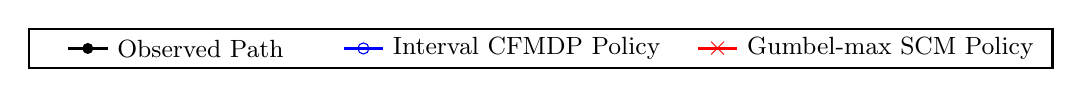
\begin{tikzpicture}[scale=1.0, every node/.style={scale=1.0}]
            \draw[thick, black] (-3, -0.25) rectangle (10, 0.25);
            %
            \draw[black, line width=1pt] (-2.5, 0.0) -- (-2,0.0);
            \fill[black] (-2.25,0.0) circle (2pt); %
            \node[right] at (-2,0.0) {\small Observed Path};
            
            %
            \draw[blue, line width=1pt] (1.0,0.0) -- (1.5,0.0);
            \node[draw=blue, circle, minimum size=4pt, inner sep=0pt] at (1.25,0.0) {}; %
            \node[right] at (1.5,0.0) {\small Interval CFMDP Policy};
            
            %
            \draw[red, line width=1pt] (5.5,0) -- (6,0);
            \node[red] at (5.75,0) {$\boldsymbol{\times}$}; %
            \node[right] at (6,0) {\small Gumbel-max SCM Policy};
        \end{tikzpicture}
    }\\
    %
    \subfigure[\footnotesize Lowest cumulative reward: Interval CFMDP ($312$), Gumbel-max SCM ($312$)]{%
        \resizebox{0.76\columnwidth}{!}{
             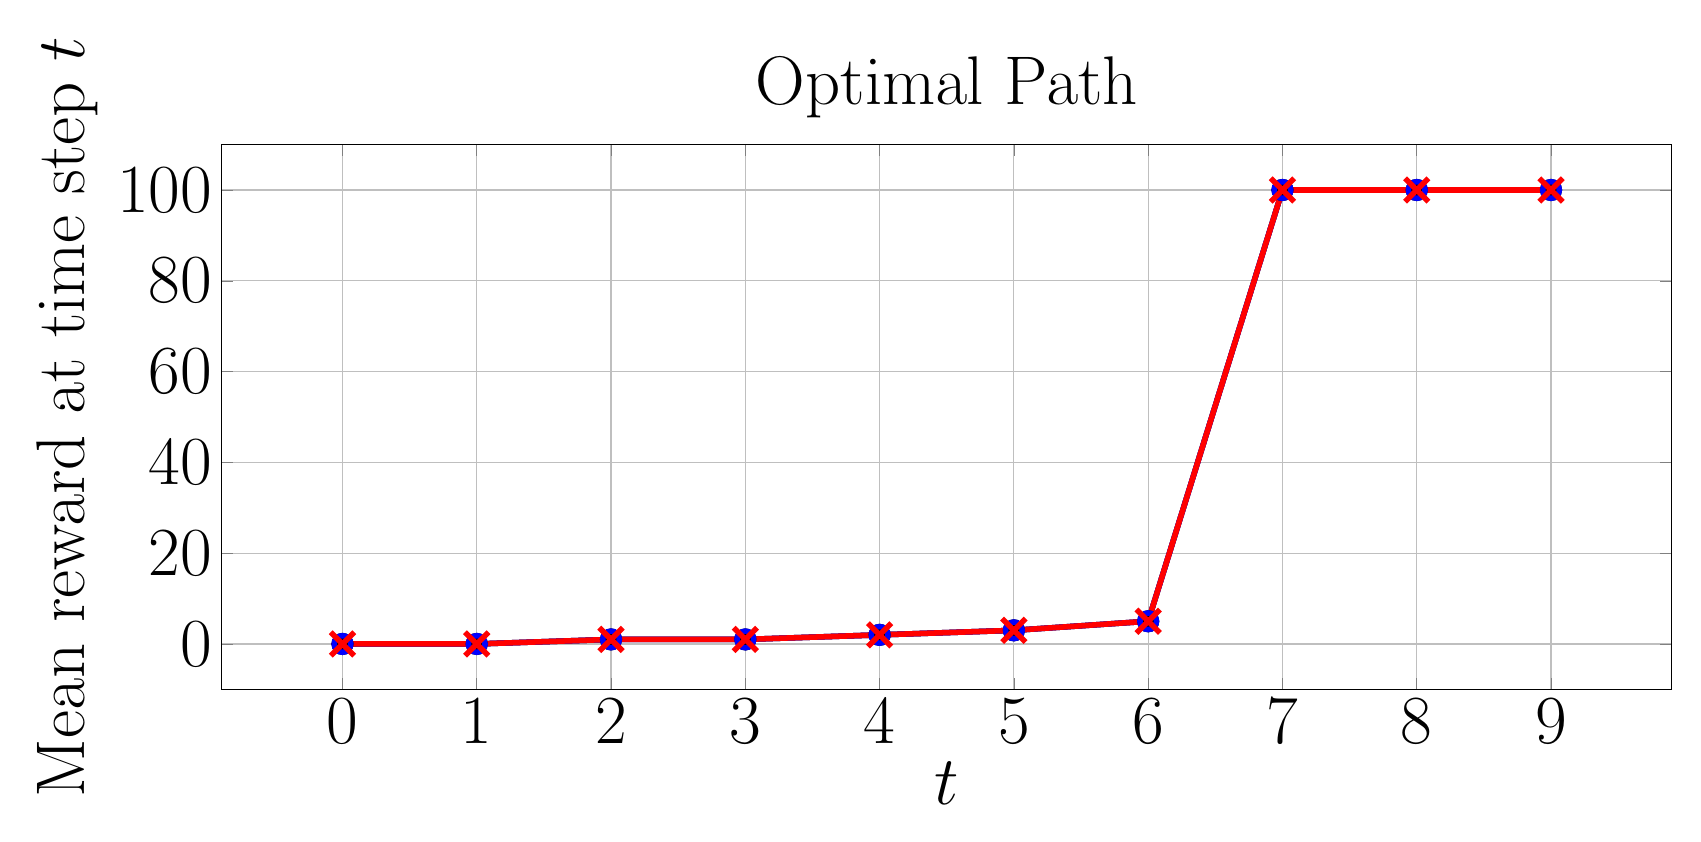
\begin{tikzpicture}
                \begin{axis}[
                    xlabel={$t$},
                    ylabel={Mean reward at time step $t$},
                    title={Optimal Path},
                    grid=both,
                    width=20cm, height=8.5cm,
                    every axis/.style={font=\Huge},
                    %
                ]
                \addplot[
                    color=black, %
                    mark=*, %
                    line width=2pt,
                    mark size=3pt,
                    error bars/.cd,
                    y dir=both, %
                    y explicit, %
                    error bar style={line width=1pt,solid},
                    error mark options={line width=1pt,mark size=4pt,rotate=90}
                ]
                coordinates {
                    (0, 0.0)  +- (0, 0.0)
                    (1, 0.0)  +- (0, 0.0) 
                    (2, 1.0)  +- (0, 0.0) 
                    (3, 1.0)  +- (0, 0.0)
                    (4, 2.0)  +- (0, 0.0)
                    (5, 3.0) +- (0, 0.0)
                    (6, 5.0) +- (0, 0.0)
                    (7, 100.0) +- (0, 0.0)
                    (8, 100.0) +- (0, 0.0)
                    (9, 100.0) +- (0, 0.0)
                };
                %
                \addplot[
                    color=blue, %
                    mark=o, %
                    line width=2pt,
                    mark size=3pt,
                    error bars/.cd,
                    y dir=both, %
                    y explicit, %
                    error bar style={line width=1pt,solid},
                    error mark options={line width=1pt,mark size=4pt,rotate=90}
                ]
                 coordinates {
                    (0, 0.0)  +- (0, 0.0)
                    (1, 0.0)  +- (0, 0.0) 
                    (2, 1.0)  +- (0, 0.0) 
                    (3, 1.0)  +- (0, 0.0)
                    (4, 2.0)  +- (0, 0.0)
                    (5, 3.0) +- (0, 0.0)
                    (6, 5.0) +- (0, 0.0)
                    (7, 100.0) +- (0, 0.0)
                    (8, 100.0) +- (0, 0.0)
                    (9, 100.0) +- (0, 0.0)
                };
                %
                \addplot[
                    color=red, %
                    mark=x, %
                    line width=2pt,
                    mark size=6pt,
                    error bars/.cd,
                    y dir=both, %
                    y explicit, %
                    error bar style={line width=1pt,solid},
                    error mark options={line width=1pt,mark size=4pt,rotate=90}
                ]
                coordinates {
                    (0, 0.0)  +- (0, 0.0)
                    (1, 0.0)  +- (0, 0.0) 
                    (2, 1.0)  +- (0, 0.0) 
                    (3, 1.0)  +- (0, 0.0)
                    (4, 2.0)  +- (0, 0.0)
                    (5, 3.0) +- (0, 0.0)
                    (6, 5.0) +- (0, 0.0)
                    (7, 100.0) +- (0, 0.0)
                    (8, 100.0) +- (0, 0.0)
                    (9, 100.0) +- (0, 0.0)
                };
                \end{axis}
            \end{tikzpicture}
         }
    }
    \hspace{1cm}
    \subfigure[\footnotesize Lowest cumulative reward: Interval CFMDP ($19$), Gumbel-max SCM ($-88$)]{%
         \resizebox{0.76\columnwidth}{!}{
            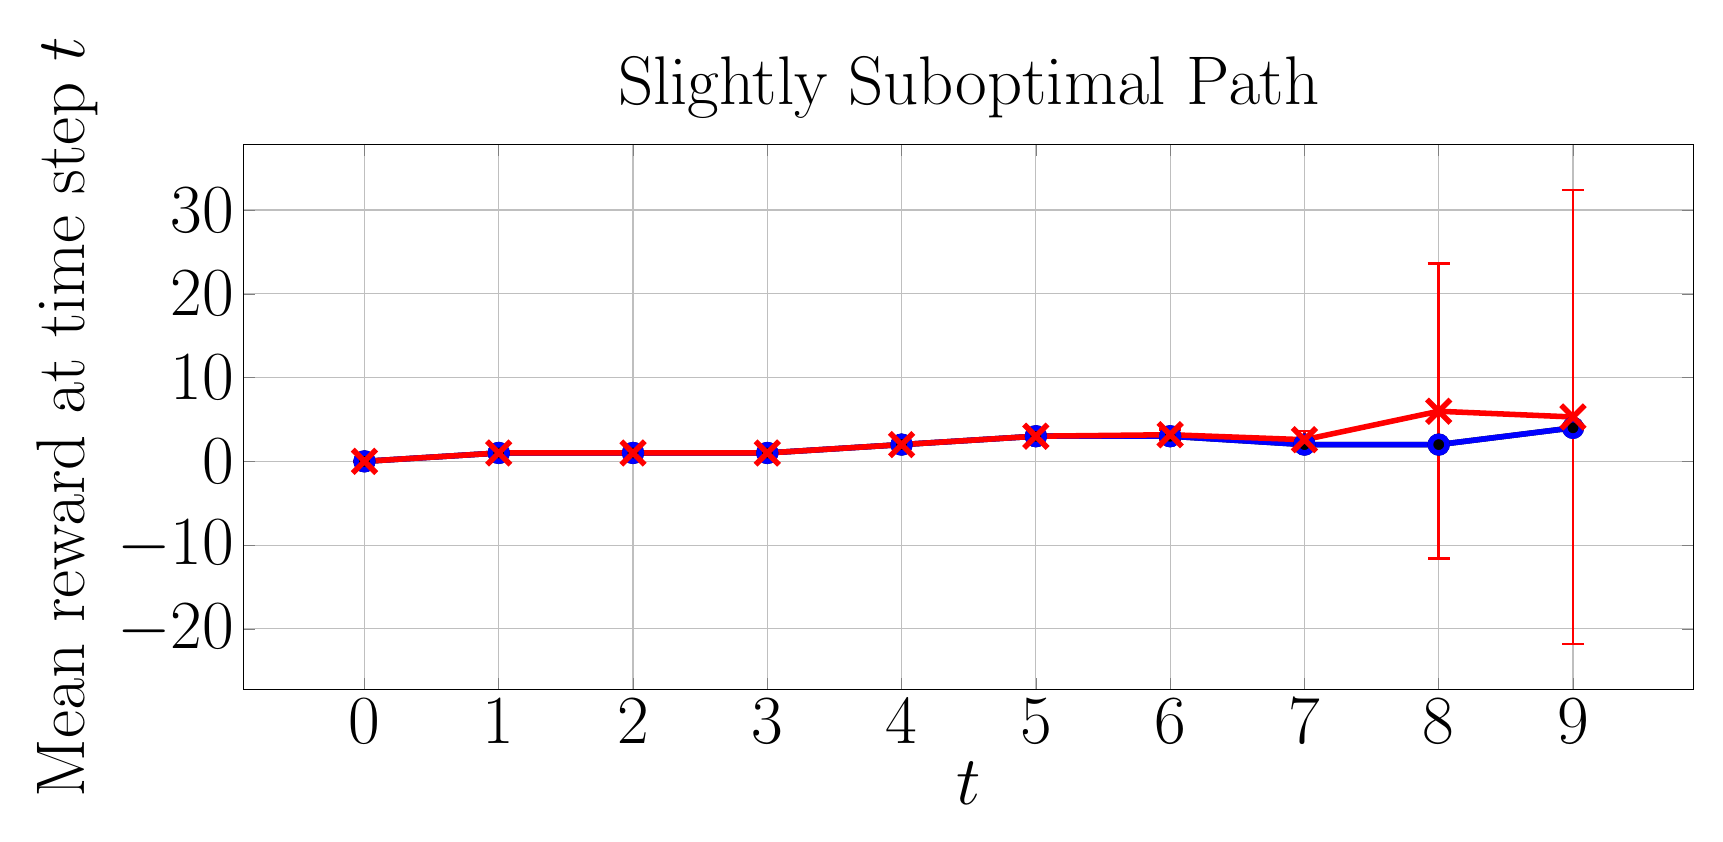
\begin{tikzpicture}
                \begin{axis}[
                    xlabel={$t$},
                    ylabel={Mean reward at time step $t$},
                    title={Slightly Suboptimal Path},
                    grid=both,
                    width=20cm, height=8.5cm,
                    every axis/.style={font=\Huge},
                    %
                ]
                \addplot[
                    color=black, %
                    mark=*, %
                    line width=2pt,
                    mark size=3pt,
                    error bars/.cd,
                    y dir=both, %
                    y explicit, %
                    error bar style={line width=1pt,solid},
                    error mark options={line width=1pt,mark size=4pt,rotate=90}
                ]
              coordinates {
                    (0, 0.0)  +- (0, 0.0)
                    (1, 1.0)  +- (0, 0.0) 
                    (2, 1.0)  +- (0, 0.0) 
                    (3, 1.0)  +- (0, 0.0)
                    (4, 2.0)  +- (0, 0.0)
                    (5, 3.0) +- (0, 0.0)
                    (6, 3.0) +- (0, 0.0)
                    (7, 2.0) +- (0, 0.0)
                    (8, 2.0) +- (0, 0.0)
                    (9, 4.0) +- (0, 0.0)
                };
                %
                \addplot[
                    color=blue, %
                    mark=o, %
                    line width=2pt,
                    mark size=3pt,
                    error bars/.cd,
                    y dir=both, %
                    y explicit, %
                    error bar style={line width=1pt,solid},
                    error mark options={line width=1pt,mark size=4pt,rotate=90}
                ]
              coordinates {
                    (0, 0.0)  +- (0, 0.0)
                    (1, 1.0)  +- (0, 0.0) 
                    (2, 1.0)  +- (0, 0.0) 
                    (3, 1.0)  +- (0, 0.0)
                    (4, 2.0)  +- (0, 0.0)
                    (5, 3.0) +- (0, 0.0)
                    (6, 3.0) +- (0, 0.0)
                    (7, 2.0) +- (0, 0.0)
                    (8, 2.0) +- (0, 0.0)
                    (9, 4.0) +- (0, 0.0)
                };
                %
                \addplot[
                    color=red, %
                    mark=x, %
                    line width=2pt,
                    mark size=6pt,
                    error bars/.cd,
                    y dir=both, %
                    y explicit, %
                    error bar style={line width=1pt,solid},
                    error mark options={line width=1pt,mark size=4pt,rotate=90}
                ]
                coordinates {
                    (0, 0.0)  +- (0, 0.0)
                    (1, 1.0)  +- (0, 0.0) 
                    (2, 1.0)  +- (0, 0.0) 
                    (3, 1.0)  +- (0, 0.0)
                    (4, 2.0)  += (0, 0.0)
                    (5, 3.0)  += (0, 0.0)
                    (6, 3.17847) += (0, 0.62606746) -= (0, 0.62606746)
                    (7, 2.5832885) += (0, 1.04598233) -= (0, 1.04598233)
                    (8, 5.978909) += (0, 17.60137623) -= (0, 17.60137623)
                    (9, 5.297059) += (0, 27.09227512) -= (0, 27.09227512)
                };
                \end{axis}
            \end{tikzpicture}
         }
    }\\[-1.5pt]
    \subfigure[\footnotesize Lowest cumulative reward: Interval CFMDP ($14$), Gumbel-max SCM ($-598$)]{%
         \resizebox{0.76\columnwidth}{!}{
             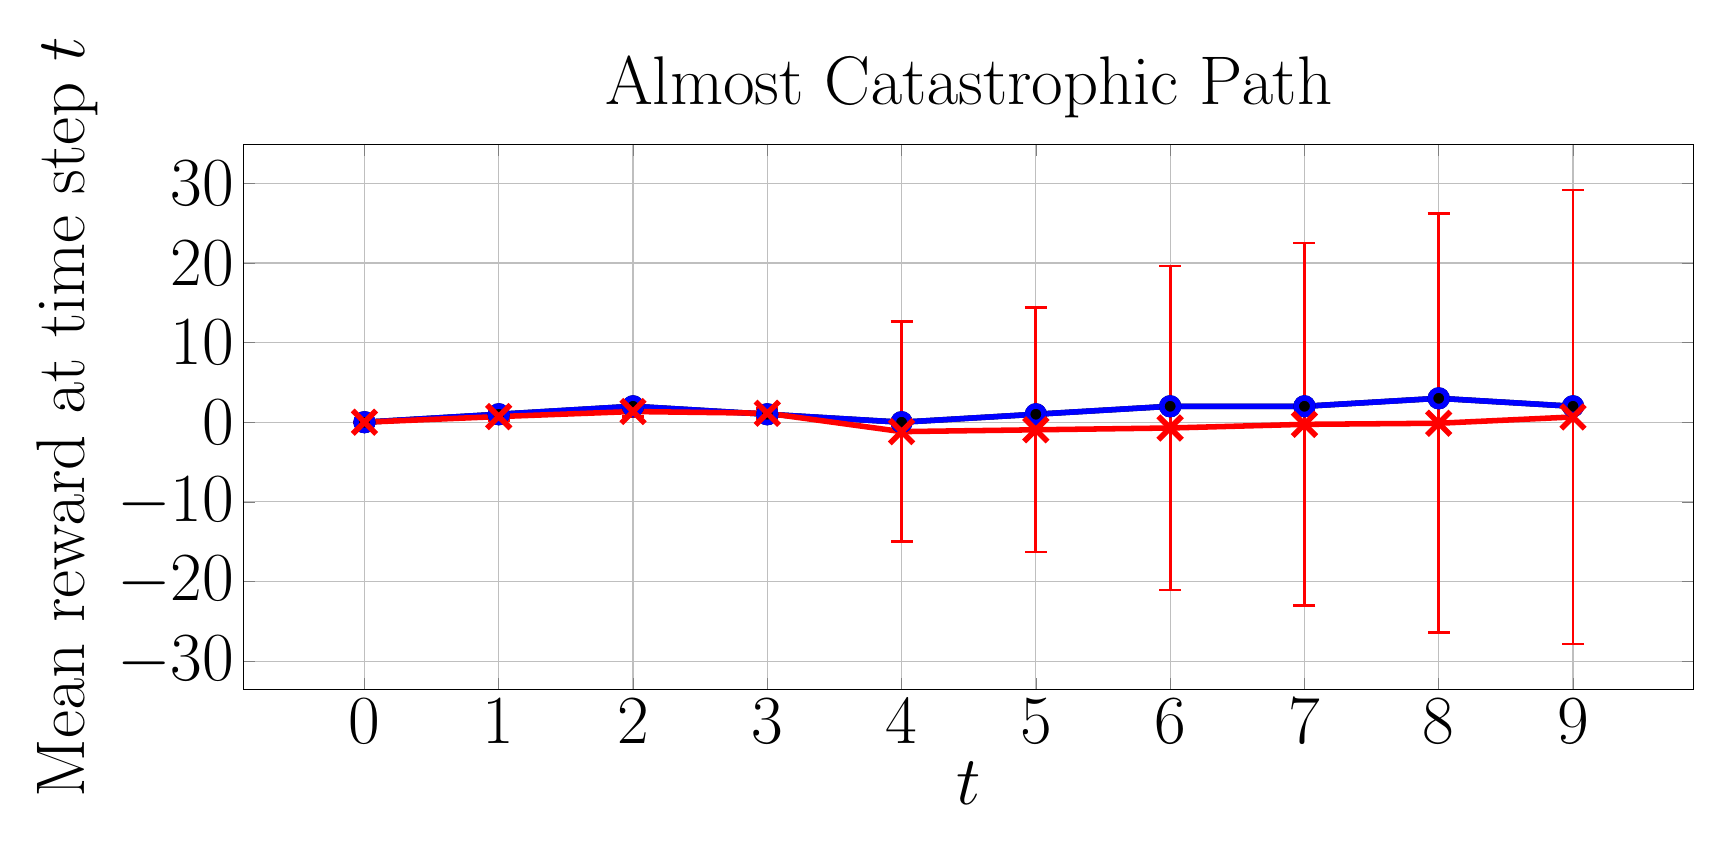
\begin{tikzpicture}
                \begin{axis}[
                    xlabel={$t$},
                    ylabel={Mean reward at time step $t$},
                    title={Almost Catastrophic Path},
                    grid=both,
                    width=20cm, height=8.5cm,
                    every axis/.style={font=\Huge},
                    %
                ]
                \addplot[
                    color=black, %
                    mark=*, %
                    line width=2pt,
                    mark size=3pt,
                    error bars/.cd,
                    y dir=both, %
                    y explicit, %
                    error bar style={line width=1pt,solid},
                    error mark options={line width=1pt,mark size=4pt,rotate=90}
                ]
                coordinates {
                    (0, 0.0)  +- (0, 0.0)
                    (1, 1.0)  +- (0, 0.0) 
                    (2, 2.0)  +- (0, 0.0) 
                    (3, 1.0)  +- (0, 0.0)
                    (4, 0.0)  +- (0, 0.0)
                    (5, 1.0) +- (0, 0.0)
                    (6, 2.0) +- (0, 0.0)
                    (7, 2.0) +- (0, 0.0)
                    (8, 3.0) +- (0, 0.0)
                    (9, 2.0) +- (0, 0.0)
                };
                %
                \addplot[
                    color=blue, %
                    mark=o, %
                    line width=2pt,
                    mark size=3pt,
                    error bars/.cd,
                    y dir=both, %
                    y explicit, %
                    error bar style={line width=1pt,solid},
                    error mark options={line width=1pt,mark size=4pt,rotate=90}
                ]
                coordinates {
                    (0, 0.0)  +- (0, 0.0)
                    (1, 1.0)  +- (0, 0.0) 
                    (2, 2.0)  +- (0, 0.0) 
                    (3, 1.0)  +- (0, 0.0)
                    (4, 0.0)  +- (0, 0.0)
                    (5, 1.0) +- (0, 0.0)
                    (6, 2.0) +- (0, 0.0)
                    (7, 2.0) +- (0, 0.0)
                    (8, 3.0) +- (0, 0.0)
                    (9, 2.0) +- (0, 0.0)
                };
                %
                \addplot[
                    color=red, %
                    mark=x, %
                    line width=2pt,
                    mark size=6pt,
                    error bars/.cd,
                    y dir=both, %
                    y explicit, %
                    error bar style={line width=1pt,solid},
                    error mark options={line width=1pt,mark size=4pt,rotate=90}
                ]
                coordinates {
                    (0, 0.0)  +- (0, 0.0)
                    (1, 0.7065655)  +- (0, 0.4553358) 
                    (2, 1.341673)  +- (0, 0.67091621) 
                    (3, 1.122926)  +- (0, 0.61281824)
                    (4, -1.1821935)  +- (0, 13.82444042)
                    (5, -0.952399)  +- (0, 15.35195457)
                    (6, -0.72672) +- (0, 20.33508414)
                    (7, -0.268983) +- (0, 22.77861454)
                    (8, -0.1310835) +- (0, 26.31013314)
                    (9, 0.65806) +- (0, 28.50670214)
                };
                %
            %
            %
            %
            %
            %
            %
            %
            %
            %
            %
            %
            %
            %
            %
            %
            %
            %
            %
                \end{axis}
            \end{tikzpicture}
         }
    }
    \hspace{1cm}
    \subfigure[\footnotesize Lowest cumulative reward: Interval CFMDP ($-698$), Gumbel-max SCM ($-698$)]{%
         \resizebox{0.76\columnwidth}{!}{
            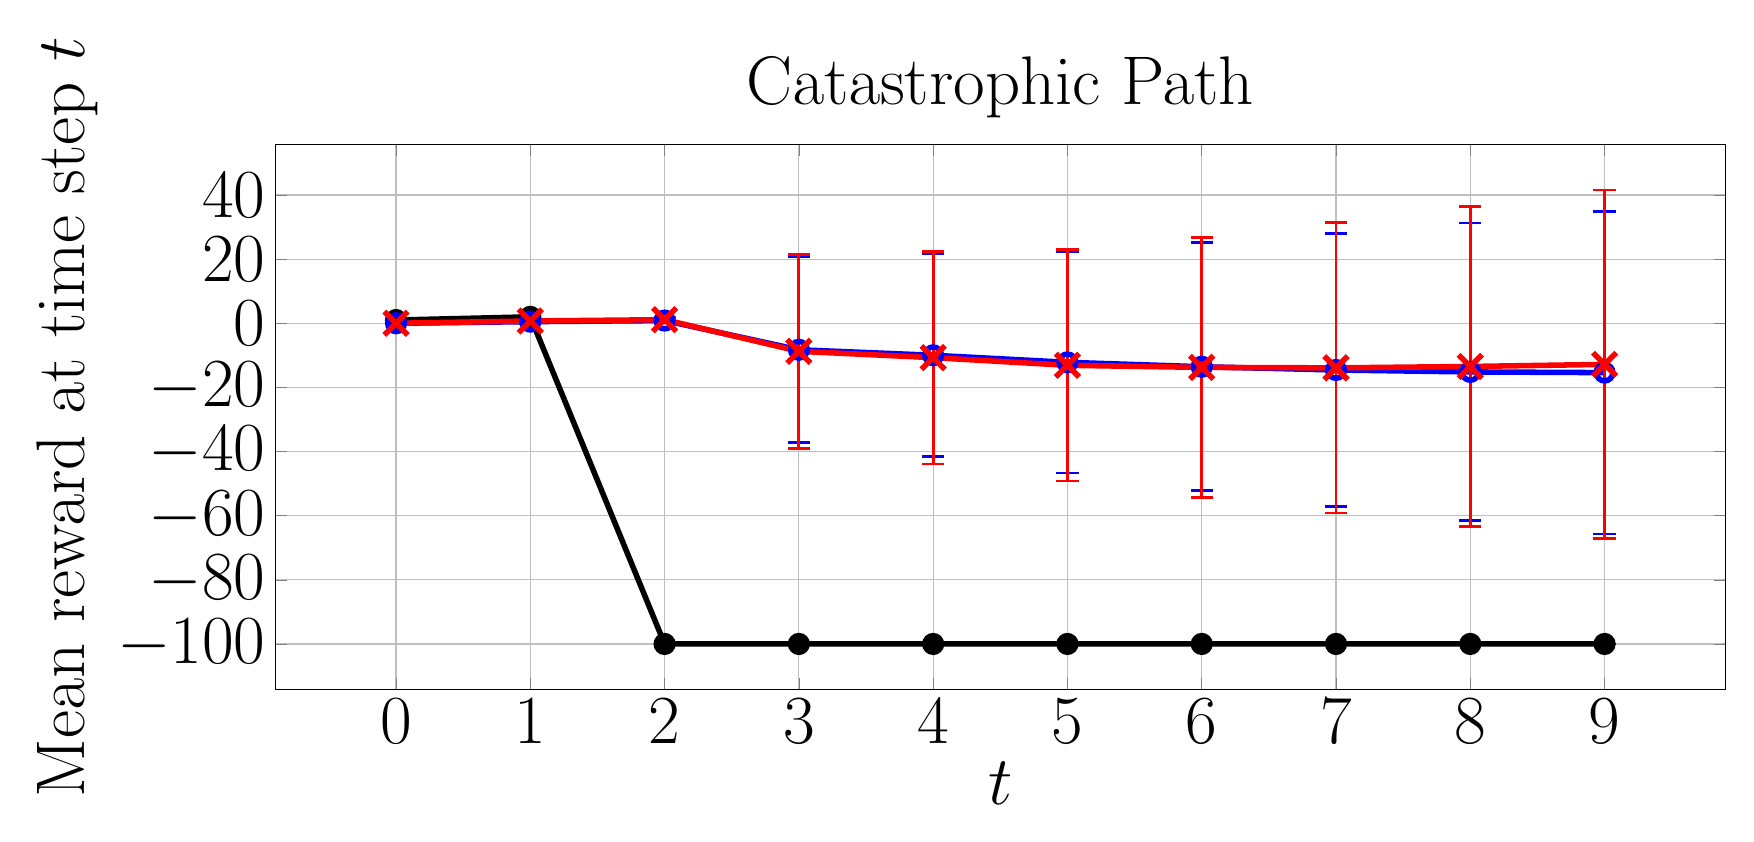
\begin{tikzpicture}
                \begin{axis}[
                    xlabel={$t$},
                    ylabel={Mean reward at time step $t$},
                    title={Catastrophic Path},
                    grid=both,
                    width=20cm, height=8.5cm,
                    every axis/.style={font=\Huge},
                    %
                ]
                \addplot[
                    color=black, %
                    mark=*, %
                    line width=2pt,
                    mark size=3pt,
                    error bars/.cd,
                    y dir=both, %
                    y explicit, %
                    error bar style={line width=1pt,solid},
                    error mark options={line width=1pt,mark size=4pt,rotate=90}
                ]
                coordinates {
                    (0, 1.0)  +- (0, 0.0)
                    (1, 2.0)  +- (0, 0.0) 
                    (2, -100.0)  +- (0, 0.0) 
                    (3, -100.0)  +- (0, 0.0)
                    (4, -100.0)  +- (0, 0.0)
                    (5, -100.0) +- (0, 0.0)
                    (6, -100.0) +- (0, 0.0)
                    (7, -100.0) +- (0, 0.0)
                    (8, -100.0) +- (0, 0.0)
                    (9, -100.0) +- (0, 0.0)
                };
                %
                \addplot[
                    color=blue, %
                    mark=o, %
                    line width=2pt,
                    mark size=3pt,
                    error bars/.cd,
                    y dir=both, %
                    y explicit, %
                    error bar style={line width=1pt,solid},
                    error mark options={line width=1pt,mark size=4pt,rotate=90}
                ]
                coordinates {
                    (0, 0.0)  +- (0, 0.0)
                    (1, 0.504814)  +- (0, 0.49997682) 
                    (2, 0.8439835)  +- (0, 0.76831917) 
                    (3, -8.2709165)  +- (0, 28.93656754)
                    (4, -9.981082)  +- (0, 31.66825363)
                    (5, -12.1776325) +- (0, 34.53463233)
                    (6, -13.556076) +- (0, 38.62845372)
                    (7, -14.574418) +- (0, 42.49603359)
                    (8, -15.1757075) +- (0, 46.41913968)
                    (9, -15.3900395) +- (0, 50.33563368)
                };
                %
                \addplot[
                    color=red, %
                    mark=x, %
                    line width=2pt,
                    mark size=6pt,
                    error bars/.cd,
                    y dir=both, %
                    y explicit, %
                    error bar style={line width=1pt,solid},
                    error mark options={line width=1pt,mark size=4pt,rotate=90}
                ]
                coordinates {
                    (0, 0.0)  +- (0, 0.0)
                    (1, 0.701873)  +- (0, 0.45743556) 
                    (2, 1.1227805)  +- (0, 0.73433129) 
                    (3, -8.7503255)  +- (0, 30.30257976)
                    (4, -10.722092)  +- (0, 33.17618589)
                    (5, -13.10721)  +- (0, 36.0648089)
                    (6, -13.7631645) +- (0, 40.56553451)
                    (7, -13.909043) +- (0, 45.23829402)
                    (8, -13.472517) +- (0, 49.96270296)
                    (9, -12.8278835) +- (0, 54.38618735)
                };
                %
            %
            %
            %
            %
            %
            %
            %
            %
            %
            %
            %
            %
            %
            %
            %
            %
            %
            %
                \end{axis}
            \end{tikzpicture}
         }
    }
    \caption{Average instant reward of CF paths induced by policies on GridWorld $p=0.4$.}
    \label{fig: reward p=0.4}
\end{figure*}

\subsection{Experimental Setup}
To compare policy performance, we measure the average rewards of counterfactual paths induced by our policy and the Gumbel-max policy by uniformly sampling $200$ counterfactual MDPs from the ICFMDP and generating $10,000$ counterfactual paths over each sampled CFMDP. \jl{Since the interval CFMDP depends on the observed path, we select $4$  paths of varying optimality to evaluate how the observed path impacts the performance of both policies: an optimal path, a slightly suboptimal path that could reach the optimal reward with a few changes, a catastrophic path that enters a catastrophic, terminal state with low reward, and an almost catastrophic path that was close to entering a catastrophic state.} When measuring the average probability bound widths and execution time needed to generate the ICFMDPs, we averaged over $20$ randomly generated observed paths
\footnote{Further training details are provided in Appendix \ref{app: training details}, and the code is provided at \href{https://github.com/ddv-lab/robust-cf-inference-in-MDPs}{https://github.com/ddv-lab/robust-cf-inference-in-MDPs}
%
%
.}.

\subsection{GridWorld}
\jl{The GridWorld MDP is a $4 \times 4$ grid where an agent must navigate from the top-left corner to the goal state in the bottom-right corner, avoiding a dangerous terminal state in the centre. At each time step, the agent can move up, down, left, or right, but there is a small probability (controlled by hyper-parameter $p$) of moving in an unintended direction. As the agent nears the goal, the reward for each state increases, culminating in a reward of $+100$ for reaching the goal. Entering the dangerous state results in a penalty of $-100$. We use two versions of GridWorld: a less stochastic version with $p=0.9$ (i.e., $90$\% chance of moving in the chosen direction) and a more stochastic version with $p=0.4$.}

\paragraph{GridWorld ($p=0.9$)}
When $p=0.9$, the counterfactual probability bounds are typically narrow (see Table \ref{tab:nonzero_probs} for average measurements). Consequently, as shown in Figure \ref{fig: reward p=0.9}, both policies are nearly identical and perform similarly well across the optimal, slightly suboptimal, and catastrophic paths.
%
However, for the almost catastrophic path, the interval CFMDP path is more conservative and follows the observed path more closely (as this is where the probability bounds are narrowest), which typically requires one additional step to reach the goal state than the Gumbel-max SCM policy.
%

\paragraph{GridWorld ($p=0.4$)}
\jl{When $p=0.4$, the GridWorld environment becomes more uncertain, increasing the risk of entering the dangerous state even if correct actions are chosen. Thus, as shown in Figure \ref{fig: reward p=0.4}, the interval CFMDP policy adopts a more conservative approach, avoiding deviation from the observed policy if it cannot guarantee higher counterfactual rewards (see the slightly suboptimal and almost catastrophic paths), whereas the Gumbel-max SCM is inconsistent: it can yield higher rewards, but also much lower rewards, reflected in the wide error bars.} For the catastrophic path, both policies must deviate from the observed path to achieve a higher reward and, in this case, perform similarly.
%
%
%
%
\subsection{Sepsis}
The Sepsis MDP \citep{oberst2019counterfactual} simulates trajectories of Sepsis patients. Each state consists of four vital signs (heart rate, blood pressure, oxygen concentration, and glucose levels), categorised as low, normal, or high.
and three treatments that can be toggled on/off at each time step (8 actions in total). Unlike \citet{oberst2019counterfactual}, we scale rewards based on the number of out-of-range vital signs, between $-1000$ (patient dies) and $1000$ (patient discharged). \jl{Like the GridWorld $p=0.4$ experiment, the Sepsis MDP is highly uncertain, as many states are equally likely to lead to optimal and poor outcomes. Thus, as shown in Figure \ref{fig: reward sepsis}, both policies follow the observed optimal and almost catastrophic paths to guarantee rewards are no worse than the observation.} However, improving the catastrophic path requires deviating from the observation. Here, the Gumbel-max SCM policy, on average, performs better than the interval CFMDP policy. But, since both policies have lower bounds clipped at $-1000$, neither policy reliably improves over the observation. In contrast, for the slightly suboptimal path, the interval CFMDP policy performs significantly better, shown by its higher lower bounds. 
Moreover, in these two cases, the worst-case counterfactual path generated by the interval CFMDP policy is better than that of the Gumbel-max SCM policy,
indicating its greater robustness.
%
\begin{figure*}
    \centering
     \resizebox{0.6\textwidth}{!}{
        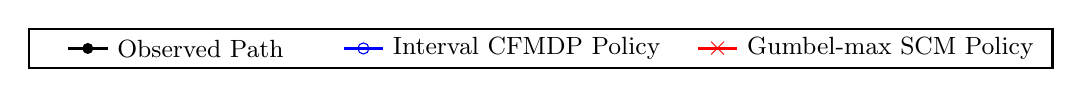
\begin{tikzpicture}[scale=1.0, every node/.style={scale=1.0}]
            \draw[thick, black] (-3, -0.25) rectangle (10, 0.25);
            %
            \draw[black, line width=1pt] (-2.5, 0.0) -- (-2,0.0);
            \fill[black] (-2.25,0.0) circle (2pt); %
            \node[right] at (-2,0.0) {\small Observed Path};
            
            %
            \draw[blue, line width=1pt] (1.0,0.0) -- (1.5,0.0);
            \node[draw=blue, circle, minimum size=4pt, inner sep=0pt] at (1.25,0.0) {}; %
            \node[right] at (1.5,0.0) {\small Interval CFMDP Policy};
            
            %
            \draw[red, line width=1pt] (5.5,0) -- (6,0);
            \node[red] at (5.75,0) {$\boldsymbol{\times}$}; %
            \node[right] at (6,0) {\small Gumbel-max SCM Policy};
        \end{tikzpicture}
    }\\
    \subfigure[\footnotesize Lowest cumulative reward: Interval CFMDP ($8000$), Gumbel-max SCM ($8000$)]{%
         \resizebox{0.76\columnwidth}{!}{
             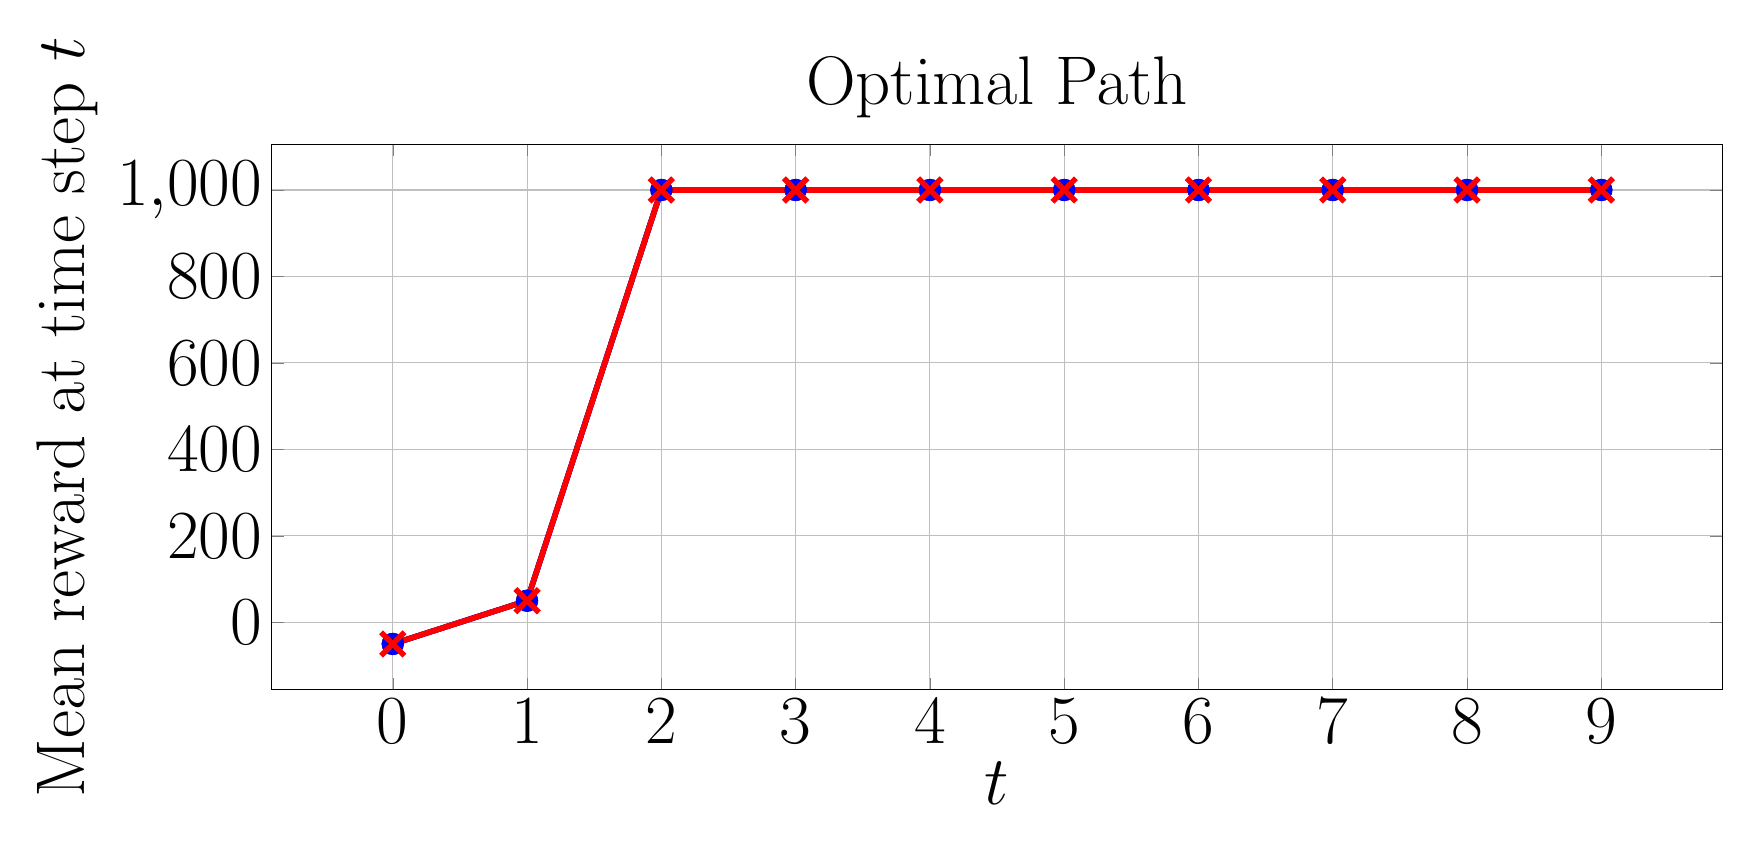
\begin{tikzpicture}
                \begin{axis}[
                    xlabel={$t$},
                    ylabel={Mean reward at time step $t$},
                    title={Optimal Path},
                    grid=both,
                    width=20cm, height=8.5cm,
                    every axis/.style={font=\Huge},
                    %
                ]
                \addplot[
                    color=black, %
                    mark=*, %
                    line width=2pt,
                    mark size=3pt,
                ]
                coordinates {
                    (0, -50.0)
                    (1, 50.0)
                    (2, 1000.0)
                    (3, 1000.0)
                    (4, 1000.0)
                    (5, 1000.0)
                    (6, 1000.0)
                    (7, 1000.0)
                    (8, 1000.0)
                    (9, 1000.0)
                };
                %
                \addplot[
                    color=blue, %
                    mark=o, %
                    line width=2pt,
                    mark size=3pt,
                    error bars/.cd,
                    y dir=both, %
                    y explicit, %
                    error bar style={line width=1pt,solid},
                    error mark options={line width=1pt,mark size=4pt,rotate=90}
                ]
                coordinates {
                    (0, -50.0)  +- (0, 0.0)
                    (1, 50.0)  +- (0, 0.0) 
                    (2, 1000.0)  +- (0, 0.0) 
                    (3, 1000.0)  +- (0, 0.0)
                    (4, 1000.0)  +- (0, 0.0)
                    (5, 1000.0) +- (0, 0.0)
                    (6, 1000.0) +- (0, 0.0)
                    (7, 1000.0) +- (0, 0.0)
                    (8, 1000.0) +- (0, 0.0)
                    (9, 1000.0) +- (0, 0.0)
                };
                %
                \addplot[
                    color=red, %
                    mark=x, %
                    line width=2pt,
                    mark size=6pt,
                    error bars/.cd,
                    y dir=both, %
                    y explicit, %
                    error bar style={line width=1pt,solid},
                    error mark options={line width=1pt,mark size=4pt,rotate=90}
                ]
                coordinates {
                    (0, -50.0)  +- (0, 0.0)
                    (1, 50.0)  +- (0, 0.0) 
                    (2, 1000.0)  +- (0, 0.0) 
                    (3, 1000.0)  +- (0, 0.0)
                    (4, 1000.0)  +- (0, 0.0)
                    (5, 1000.0) +- (0, 0.0)
                    (6, 1000.0) +- (0, 0.0)
                    (7, 1000.0) +- (0, 0.0)
                    (8, 1000.0) +- (0, 0.0)
                    (9, 1000.0) +- (0, 0.0)
                };
                %
                \end{axis}
            \end{tikzpicture}
         }
    }
    \hspace{1cm}
    \subfigure[\footnotesize Lowest cumulative reward: Interval CFMDP ($-5980$), Gumbel-max SCM ($-8000$)]{%
         \resizebox{0.76\columnwidth}{!}{
            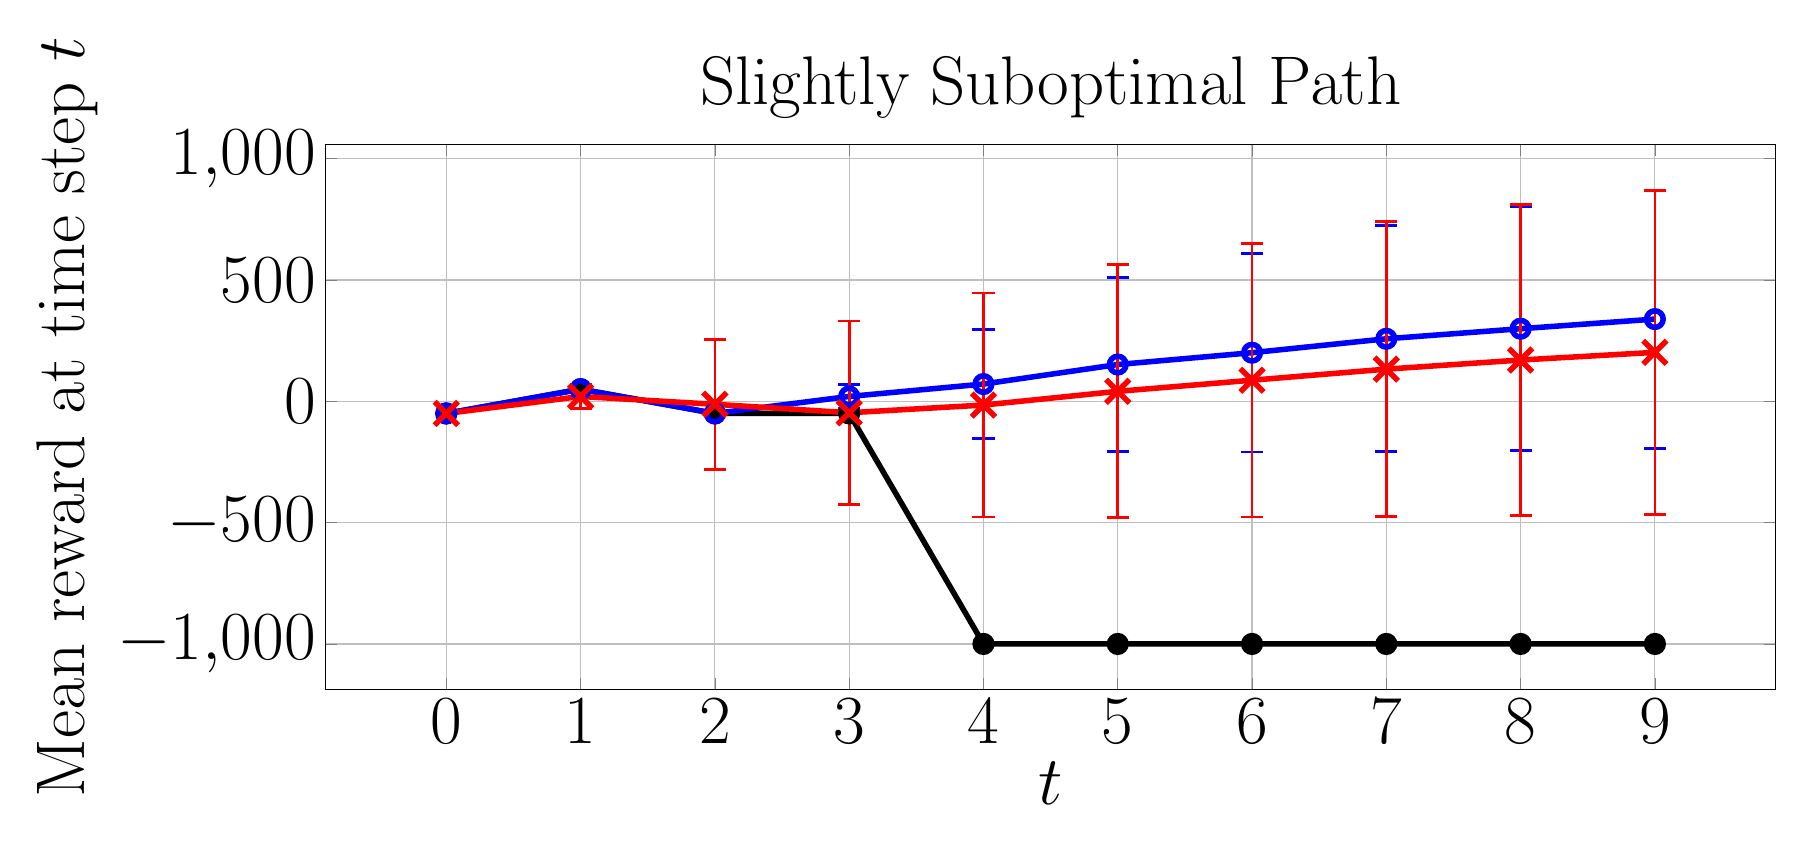
\begin{tikzpicture}
                \begin{axis}[
                    xlabel={$t$},
                    ylabel={Mean reward at time step $t$},
                    title={Slightly Suboptimal Path},
                    grid=both,
                    width=20cm, height=8.5cm,
                    every axis/.style={font=\Huge},
                    %
                ]
               \addplot[
                    color=black, %
                    mark=*, %
                    line width=2pt,
                    mark size=3pt,
                ]
                coordinates {
                    (0, -50.0)
                    (1, 50.0)
                    (2, -50.0)
                    (3, -50.0)
                    (4, -1000.0)
                    (5, -1000.0)
                    (6, -1000.0)
                    (7, -1000.0)
                    (8, -1000.0)
                    (9, -1000.0)
                };
                %
                \addplot[
                    color=blue, %
                    mark=o, %
                    line width=2pt,
                    mark size=3pt,
                    error bars/.cd,
                    y dir=both, %
                    y explicit, %
                    error bar style={line width=1pt,solid},
                    error mark options={line width=1pt,mark size=4pt,rotate=90}
                ]
                coordinates {
                    (0, -50.0)  +- (0, 0.0)
                    (1, 50.0)  +- (0, 0.0) 
                    (2, -50.0)  +- (0, 0.0) 
                    (3, 20.0631)  +- (0, 49.97539413)
                    (4, 71.206585)  +- (0, 226.02033693)
                    (5, 151.60797) +- (0, 359.23292559)
                    (6, 200.40593) +- (0, 408.86185176)
                    (7, 257.77948) +- (0, 466.10372804)
                    (8, 299.237465) +- (0, 501.82579506)
                    (9, 338.9129) +- (0, 532.06124996)
                };
                %
                \addplot[
                    color=red, %
                    mark=x, %
                    line width=2pt,
                    mark size=6pt,
                    error bars/.cd,
                    y dir=both, %
                    y explicit, %
                    error bar style={line width=1pt,solid},
                    error mark options={line width=1pt,mark size=4pt,rotate=90}
                ]
                coordinates {
                    (0, -50.0)  +- (0, 0.0)
                    (1, 20.00736)  +- (0, 49.99786741) 
                    (2, -12.282865)  +- (0, 267.598755) 
                    (3, -47.125995)  +- (0, 378.41755832)
                    (4, -15.381965)  +- (0, 461.77616558)
                    (5, 41.15459) +- (0, 521.53189262)
                    (6, 87.01595) +- (0, 564.22243126 )
                    (7, 132.62376) +- (0, 607.31338037)
                    (8, 170.168145) +- (0, 641.48013693)
                    (9, 201.813135) +- (0, 667.29441777)
                };
                %
                %
                %
                %
                %
                %
                %
                %
                %
                %
                %
                %
                %
                %
                %
                %
                %
                %
                %
                \end{axis}
            \end{tikzpicture}
         }
    }\\[-1.5pt]
    \subfigure[\footnotesize Lowest cumulative reward: Interval CFMDP ($100$), Gumbel-max SCM ($100$)]{%
         \resizebox{0.76\columnwidth}{!}{
             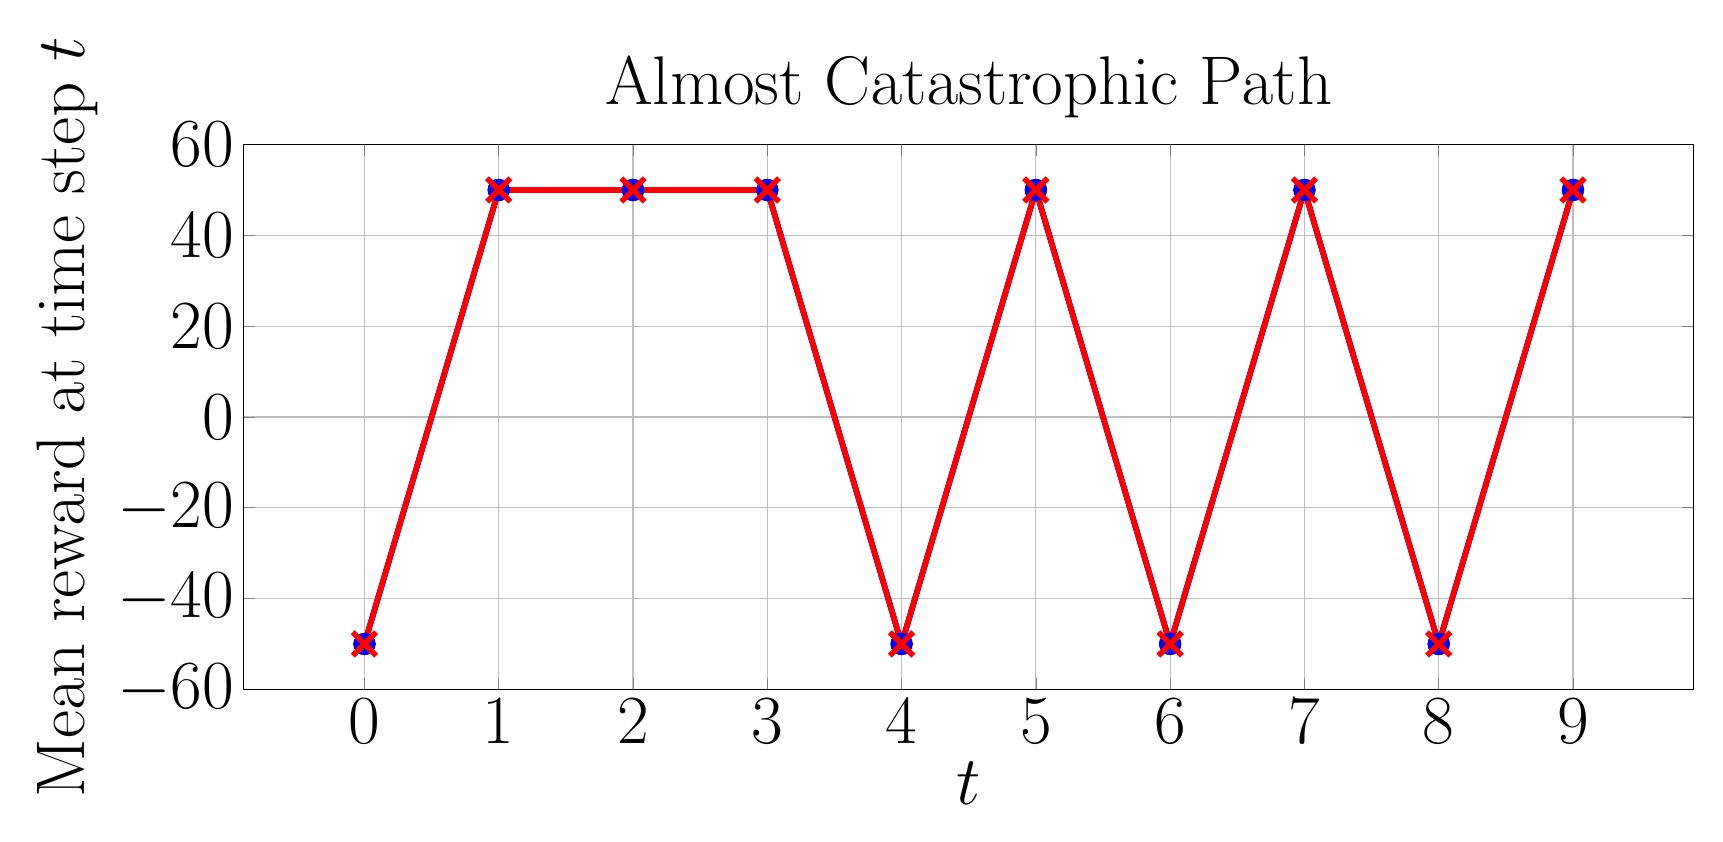
\begin{tikzpicture}
                \begin{axis}[
                    xlabel={$t$},
                    ylabel={Mean reward at time step $t$},
                    title={Almost Catastrophic Path},
                    grid=both,
                    every axis/.style={font=\Huge},
                    width=20cm, height=8.5cm,
                    %
                ]
               \addplot[
                    color=black, %
                    mark=*, %
                    line width=2pt,
                    mark size=3pt,
                ]
                coordinates {
                    (0, -50.0)
                    (1, 50.0)
                    (2, 50.0)
                    (3, 50.0)
                    (4, -50.0)
                    (5, 50.0)
                    (6, -50.0)
                    (7, 50.0)
                    (8, -50.0)
                    (9, 50.0)
                };
                %
                %
                \addplot[
                    color=blue, %
                    mark=o, %
                    line width=2pt,
                    mark size=3pt,
                    error bars/.cd,
                    y dir=both, %
                    y explicit, %
                    error bar style={line width=1pt,solid},
                    error mark options={line width=1pt,mark size=4pt,rotate=90}
                ]
                coordinates {
                    (0, -50.0)  +- (0, 0.0)
                    (1, 50.0)  +- (0, 0.0) 
                    (2, 50.0)  +- (0, 0.0) 
                    (3, 50.0)  +- (0, 0.0)
                    (4, -50.0)  +- (0, 0.0)
                    (5, 50.0) +- (0, 0.0)
                    (6, -50.0) +- (0, 0.0)
                    (7, 50.0) +- (0, 0.0)
                    (8, -50.0) +- (0, 0.0)
                    (9, 50.0) +- (0, 0.0)
                };
                %
                \addplot[
                    color=red, %
                    mark=x, %
                    line width=2pt,
                    mark size=6pt,
                    error bars/.cd,
                    y dir=both, %
                    y explicit, %
                    error bar style={line width=1pt,solid},
                    error mark options={line width=1pt,mark size=4pt,rotate=90}
                ]
                coordinates {
                    (0, -50.0)  +- (0, 0.0)
                    (1, 50.0)  +- (0, 0.0) 
                    (2, 50.0)  +- (0, 0.0) 
                    (3, 50.0)  +- (0, 0.0)
                    (4, -50.0)  +- (0, 0.0)
                    (5, 50.0) +- (0, 0.0)
                    (6, -50.0) +- (0, 0.0)
                    (7, 50.0) +- (0, 0.0)
                    (8, -50.0) +- (0, 0.0)
                    (9, 50.0) +- (0, 0.0)
                };
                %
                %
                %
                %
                %
                %
                %
                %
                %
                %
                %
                %
                %
                %
                %
                %
                %
                %
                %
                \end{axis}
            \end{tikzpicture}
         }
    }
    \hspace{1cm}
    \subfigure[\footnotesize Lowest cumulative reward: Interval CFMDP ($-7150$), Gumbel-max SCM ($-9050$)]{%
         \resizebox{0.76\columnwidth}{!}{
            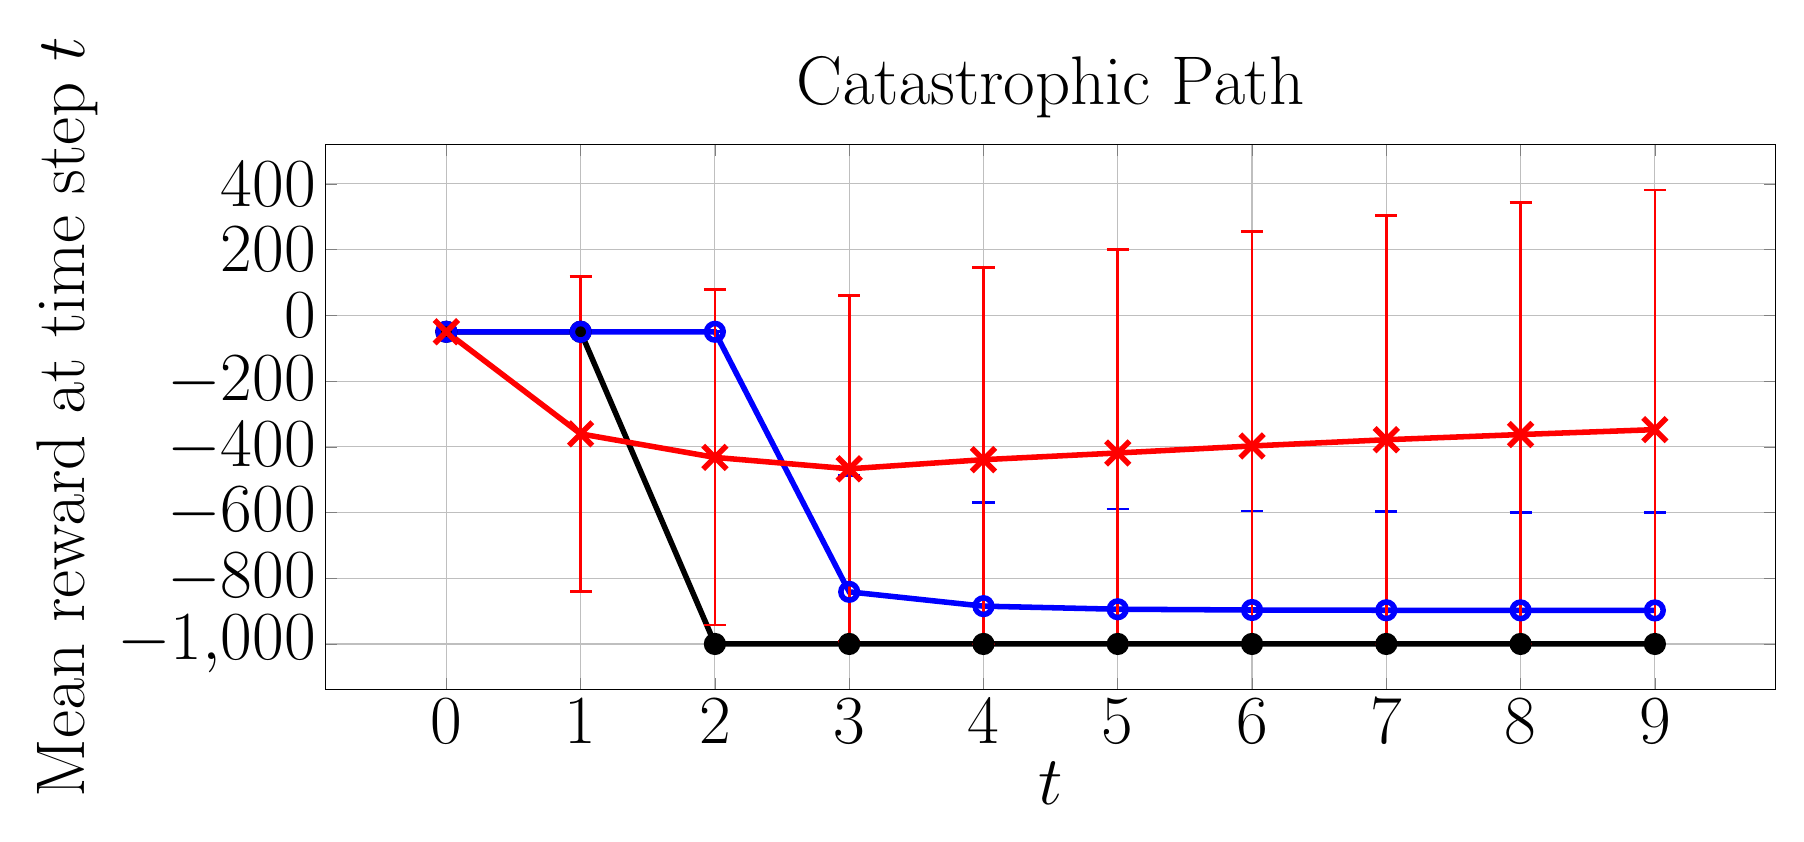
\begin{tikzpicture}
                \begin{axis}[
                    xlabel={$t$},
                    ylabel={Mean reward at time step $t$},
                    title={Catastrophic Path},
                    grid=both,
                    width=20cm, height=8.5cm,
                    every axis/.style={font=\Huge},
                    %
                ]
               \addplot[
                    color=black, %
                    mark=*, %
                    line width=2pt,
                    mark size=3pt,
                ]
                coordinates {
                    (0, -50.0)
                    (1, -50.0)
                    (2, -1000.0)
                    (3, -1000.0)
                    (4, -1000.0)
                    (5, -1000.0)
                    (6, -1000.0)
                    (7, -1000.0)
                    (8, -1000.0)
                    (9, -1000.0)
                };
                %
                %
                \addplot[
                    color=blue, %
                    mark=o, %
                    line width=2pt,
                    mark size=3pt,
                    error bars/.cd,
                    y dir=both, %
                    y explicit, %
                    error bar style={line width=1pt,solid},
                    error mark options={line width=1pt,mark size=4pt,rotate=90}
                ]
                coordinates {
                    (0, -50.0)  +- (0, 0.0)
                    (1, -50.0)  +- (0, 0.0) 
                    (2, -50.0)  +- (0, 0.0) 
                    (3, -841.440725)  += (0, 354.24605512) -= (0, 158.559275)
                    (4, -884.98225)  += (0, 315.37519669) -= (0, 115.01775)
                    (5, -894.330425) += (0, 304.88572805) -= (0, 105.669575)
                    (6, -896.696175) += (0, 301.19954514) -= (0, 103.303825)
                    (7, -897.4635) += (0, 299.61791279) -= (0, 102.5365)
                    (8, -897.77595) += (0, 298.80392585) -= (0, 102.22405)
                    (9, -897.942975) += (0, 298.32920557) -= (0, 102.057025)
                };
                %
                \addplot[
                    color=red, %
                    mark=x, %
                    line width=2pt,
                    mark size=6pt,
                    error bars/.cd,
                    y dir=both, %
                    y explicit, %
                    error bar style={line width=1pt,solid},
                    error mark options={line width=1pt,mark size=4pt,rotate=90}
                ]
            coordinates {
                    (0, -50.0)  +- (0, 0.0)
                    (1, -360.675265)  +- (0, 479.39812699) 
                    (2, -432.27629)  +- (0, 510.38620897) 
                    (3, -467.029545)  += (0, 526.36009628) -= (0, 526.36009628)
                    (4, -439.17429)  += (0, 583.96638919) -= (0, 560.82571)
                    (5, -418.82704) += (0, 618.43027478) -= (0, 581.17296)
                    (6, -397.464895) += (0, 652.67322574) -= (0, 602.535105)
                    (7, -378.49052) += (0, 682.85407033) -= (0, 621.50948)
                    (8, -362.654195) += (0, 707.01412023) -= (0, 637.345805)
                    (9, -347.737935) += (0, 729.29076479) -= (0, 652.262065)
                };
                %
                %
                %
                %
                %
                %
                %
                %
                %
                %
                %
                %
                %
                %
                %
                %
                %
                %
                %
                \end{axis}
            \end{tikzpicture}
         }
    }
    \caption{Average instant reward of CF paths induced by policies on Sepsis.}
    \label{fig: reward sepsis}
\end{figure*}

%
%
%
\subsection{Interval CFMDP Bounds}
%
%
Table \ref{tab:nonzero_probs} presents the mean counterfactual probability bound widths (excluding transitions where the upper bound is $0$) for each MDP, averaged over 20 observed paths. We compare the bounds under counterfactual stability (CS) and monotonicity (M) assumptions, CS alone, and no assumptions. This shows that the assumptions marginally reduce the bound widths, indicating the assumptions tighten the bounds without excluding too many causal models, as intended.
\renewcommand{\arraystretch}{1}

\begin{table}
\centering
\caption{Mean width of counterfactual probability bounds}
\resizebox{0.8\columnwidth}{!}{%
\begin{tabular}{|c|c|c|c|}
\hline
\multirow{2}{*}{\textbf{Environment}} & \multicolumn{3}{c|}{\textbf{Assumptions}} \\ \cline{2-4}
 & \textbf{CS + M} & \textbf{CS} & \textbf{None\tablefootnote{\jl{Equivalent to \citet{li2024probabilities}'s bounds (see Section \ref{sec: equivalence with Li}).}}} \\ \hline
\textbf{GridWorld} ($p=0.9$) & 0.0817 & 0.0977 & 0.100 \\ \hline
\textbf{GridWorld} ($p=0.4$) & 0.552  & 0.638  & 0.646 \\ \hline
\textbf{Sepsis} & 0.138 & 0.140 & 0.140 \\ \hline
\end{tabular}
}
\label{tab:nonzero_probs}
\end{table}


\subsection{Execution Times}
Table \ref{tab: times} compares the average time needed to generate the interval CFMDP vs.\ the Gumbel-max SCM CFMDP for 20 observations.
The GridWorld algorithms were run single-threaded, while the Sepsis experiments were run in parallel.
Generating the interval CFMDP is significantly faster as it uses exact analytical bounds, whereas the Gumbel-max CFMDP requires sampling from the Gumbel distribution to estimate counterfactual transition probabilities. \jl{Since constructing the counterfactual MDP models is the main bottleneck in both approaches, ours is more efficient overall and suitable for larger MDPs.}
\begin{table}
\centering
\caption{Mean execution time to generate CFMDPs}
\resizebox{0.99\columnwidth}{!}{%
\begin{tabular}{|c|c|c|}
\hline
\multirow{2}{*}{\textbf{Environment}} & \multicolumn{2}{c|}{\textbf{Mean Execution Time (s)}} \\ \cline{2-3} 
                                      & \textbf{Interval CFMDP} & \textbf{Gumbel-max CFMDP} \\ \hline
\textbf{GridWorld ($p=0.9$) }                  & 0.261                   & 56.1                      \\ \hline
\textbf{GridWorld ($p=0.4$)  }                 & 0.336                   & 54.5                      \\ \hline
\textbf{Sepsis}                                 & 688                     & 2940                      \\ \hline
\end{tabular}%
}
\label{tab: times}
\end{table}



